\chapter{Testing and Evaluation}

Since this project concerns a novel concept, the testing procedure was primarily aimed at demonstrating some level of accuracy in predicting the items of data that a specific user would want to see at a given time of day.

\section{Test Environment}

In order to efficiently create and manage test data and to observe the output of the ranking algorithm, a testing environment was implemented as a wrapper program around the API. This is a Java command-line application which enables test \emph{DataItems} to be entered by hand and stored in an organised JSON object database.

A file manager class (\emph{FileManager}) was developed to store static methods for reading to and writing from text files. A test data manager class (\emph{TestDataManager}) was created which manages test data creation for each of the available types of data items; directory scanning for finding subsets of the test data and the loading of test data items, and of specific sets of data items.

\section{Verification Strategy}

The primary criteria by which the effectiveness of the recommender system is assessed is the extent to which it is able to predict the order of relevance of items data that a specific user wants to see. 8 individuals completed a questionnaire in which they were asked to manually order 3 sets of 10 items of data from a range of sources into their order of interest. They also recorded their personality profile which denoted their relative interests in 12 topics. 

\subsection{Test data}

Test data was acquired from 30 genuine sources from a range of authors to give a maximum representation of the wide range of styles, quality and topics of items of social media and productivity-related data. There was a total of 8 respondents, each ranking 3 sets of 10 items. This was considered a sufficient number to extract reliable information concerning accuracy, since the probability of an apparent trend from 24 (number of manually ordered lists) responses being due to chance is negligible. In addition 24 responses provides sufficient clarity to determine the extent of any degree of agreement, not just whether one exists. 

\subsection{Kendall's $\tau$ Coefficient for Agreement}

Kendall's $\tau$ correlation coefficient is a statistical measure of agreement between two lists of measured quantities. It is a particular case of a generalised correlation coefficient discovered by Kendall (1944) (Eqn. \ref{GeneralisedForm}) which gives a score to any set of two properties. 

\begin{equation}\label{GeneralisedForm}	
	\Gamma  = \frac{\sum_{i,j=1}^{n}a_{ij}b_{ij}}{\sqrt{\sum_{i,j=1}^{n}a_{ij}^2\sum_{i,j=1}^{n}b_{ij}^2}} 
\end{equation}

Stated in equation \ref{KendallsTau}, Kendall's $\tau$ is based on the difference between the number of concordant pairs $n_c$ and the number of discordant pairs $n_d$. $n_c$ is the number of ranks (positions in list) below the $i^{th}$ rank which have a larger value than that particular rank. Similarly, $n_d$ is the number of observed ranks below the $i^{th}$ rank which have a smaller value than that particular rank. Consequently, two ordered lists in perfect agreement have no discordant pairs since all of the proceeding ranks from a given rank have values lower than that particular rank. 

\begin{equation}\label{KendallsTau}	
	\tau  = \frac{n_c - n_d}{n_c+n_d} 
\end{equation}

Kendall's $\tau = \{-1, 1\}$ is used in the testing of the recommender system as a measure of the extent to which the order of relevance of the outputted items of data, match the order of the manually sorted list of items of data. $\tau = -1$ indicates complete disagreement in the order of the two lists of items (the second is a reversal of the first) and $\tau = 1$ indicates complete agreement. A value of $0$ is indicative of a pair of lists with no apparent level of agreement or disagreement as would be expected from two randomly ordered lists of integers with the same range.  

This form of Kendall's $\tau$ is influenced less by the presence of a low number of pairs extremely different in value. This better suits the validation of a problem such as a recommender system since a single value incorrect by a large amount among other pairs which are more or less accurate, would otherwise yield a higher value of $\tau$ thus distorting the output to a lesser extent. 

\subsection{Key assumptions and limitations}

The primary assumption to be considered when approaching this method of the verification of test results, is the assumption that a perfect recommender system would rank items of data in the precise order that the user would manually rank them. This is not necessarily the case, since a user may not want to see the items most \textit{relevant} to them, but the items most \textit{interesting} or \textit{enjoyable} which is not the goal of the algorithm. 

This method of verification is limited in its reliance upon the correct manual ordering of items by the user, since due to a users minor misunderstanding of our criteria of relevance or slight carelessness, the manually ordered list is unlikely to perfectly represent the users actual order of relevance of items. 

The limited size of 10 of the sets of test data presents a limitation on the test procedure, since there may be a greater degree of accuracy for larger lists however it is large enough to remove the likelihood of chance-based agreement. 

\section{Kendall's $\tau$}

In order to get a picture of the accuracy of the algorithm, Kendall's $\tau$ was used to measure the level of agreement between the output and the manually ordered lists of test items. For each of the 3 ranked sets for each of the 8 respondents $\tau$ was calculated using the corresponding output from the API. Figure \ref{kendallsTauGraph} shows these values as frequency against $\tau$. 

\begin{figure}[ht!]
    \makebox[\linewidth]{
       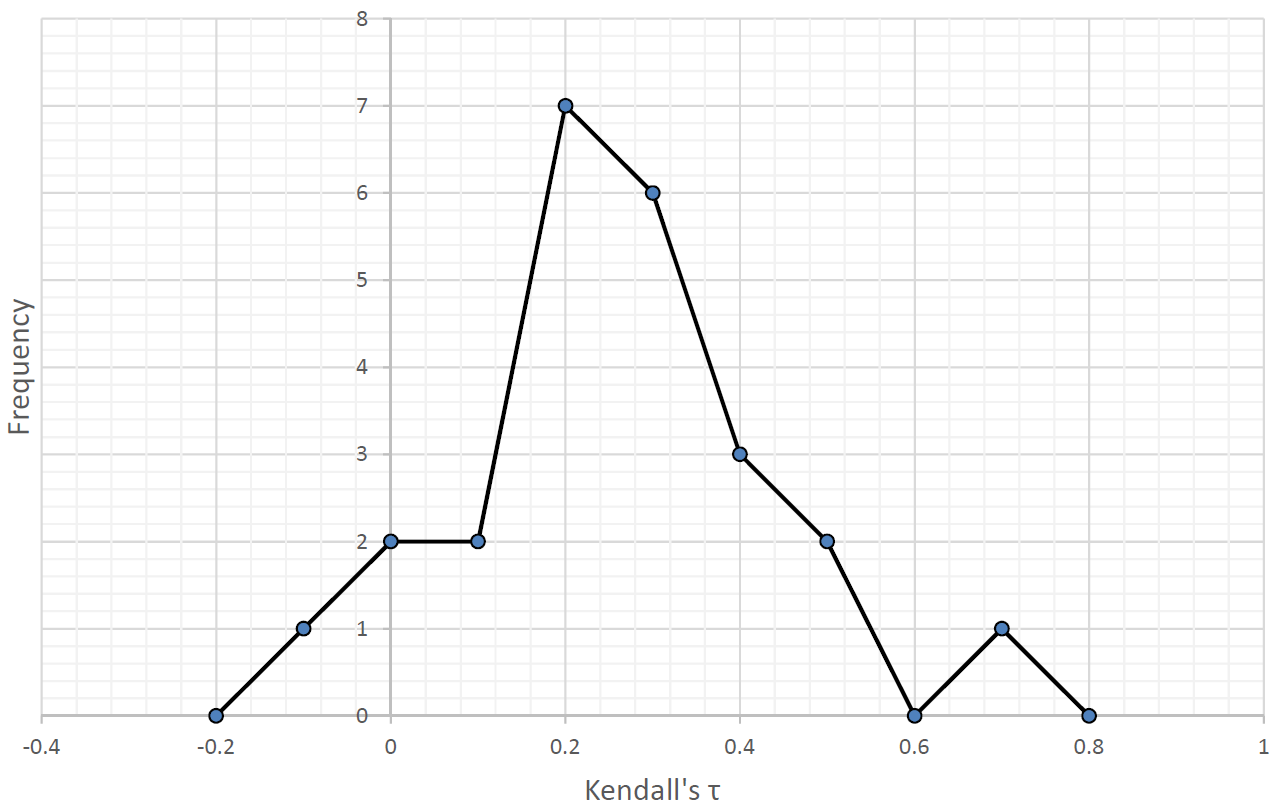
\includegraphics[width=1.0\linewidth]{images/graph1.png}
    }
    \caption{Kendall's $\tau$ distribution of all data types}
    \label{kendallsTauGraph}
\end{figure}

The mean value of $\tau$ for the data in figure \ref{kendallsTauGraph} is \textbf{0.205} which indicates that there is somewhat agreement between the predicted order of relevance of items and their true values. However, since agreement is measured from $\tau = 0$ to $\tau = 1$, there is significant room for improvement. 

One of the trends that the verification stage revealed was that users typically ordered tasks and appointments as their first and second priority items. Due to the design of the algorithm, such types of data are scored based upon the time until their due date and are consistently scored more highly than any item of social media. It therefore became clear that a significant portion of this apparent agreement may have been primarily due to the ordering of types of item, rather than topics of items within types.

Figure \ref{kendallsTauGraph2} shows the frequency distribution of the values of $\tau$ when considering only the items of social media. This was done in order to eliminate the agreement between types of items and focus on the extent to which topic is able to predict relevance. 

\begin{figure}[ht!]
    \makebox[\linewidth]{
       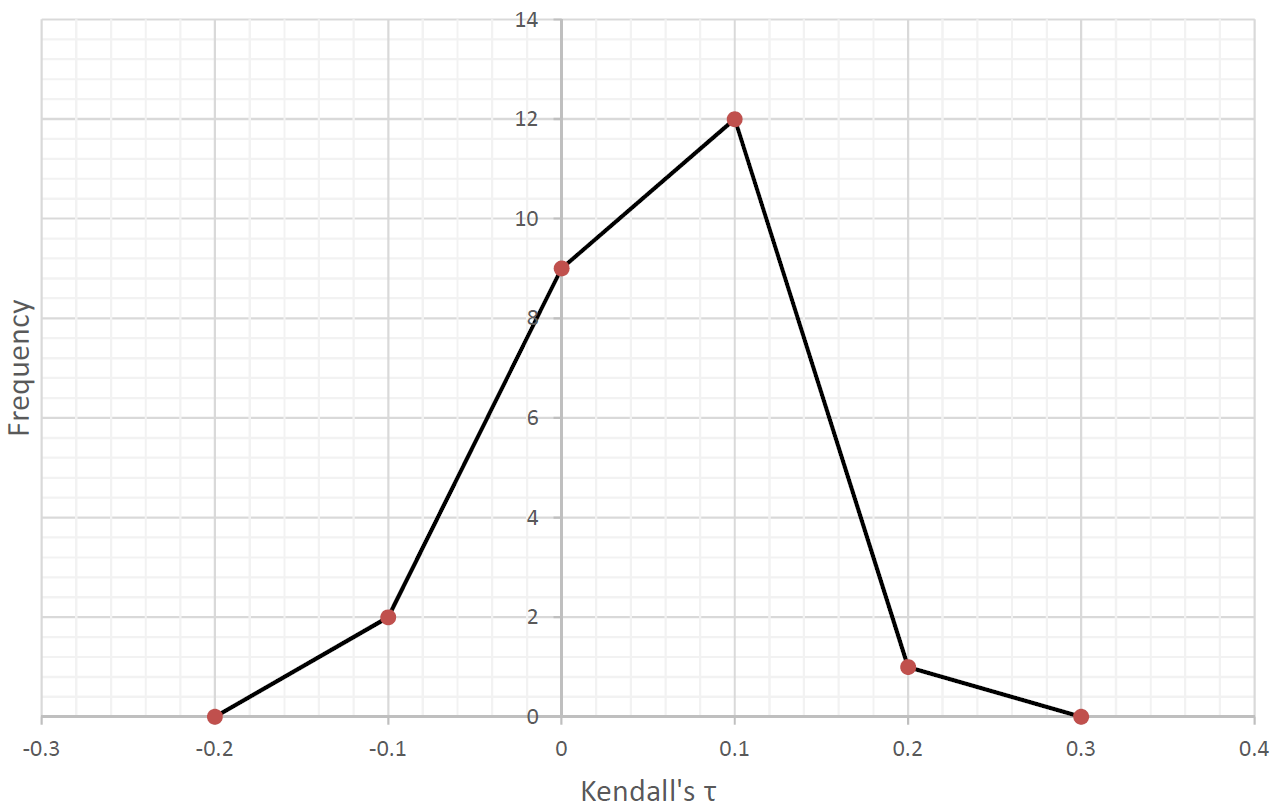
\includegraphics[width=1.0\linewidth]{images/graph2.png}
    }
    \caption{Kendall's $\tau$ distribution of social media}
    \label{kendallsTauGraph2}
\end{figure}

The results of this calculation show that there is no significant agreement between the two ordered lists which indicates that the algorithm has little predictive power in recommending items based upon topic. 

The most obvious reasons for this are \emph{a)} that unlike news and entertainment, the topic of an item is not a good indicator of relevance when dealing specifically with social media, \emph{b)} the uncertainty involved in the correct topic classification of the items using the DatumBox service, and \emph{c)} the limited classes (topics) which an item can fall into, leading to a weakly justified connection between an attribute of the the user profile and the items topic.
